\documentclass[12pt,a4paper]{article}
\usepackage[ngerman]{babel}
\usepackage[utf8]{inputenc}
\usepackage[unicode=true,bookmarks=false,bookmarksopen=true]{hyperref}

\usepackage{xcolor}
\usepackage{graphicx}
\usepackage{tikz}

\def\checkmark{\tikz\fill[scale=0.4](0,.35) -- (.25,0) -- (1,.7) -- (.25,.15) -- cycle;}

\title{ORES Preparation IV}
\author{Tom Gülenman}
\begin{document}
\maketitle
\textit{Disclaimer: No guarantee for the correctness of information / explanations / sources is given.}\\
%
\section*{Goals}
\begin{enumerate}
\item Adjust crucial metrics list to match the damaging model metrics
\item Check out mail attachments
\item Check out new Confluence pages and goals
\item Research
\begin{itemize}
\item Check out FAT Conference Docs
\item In what other cases than confusion matrices are those parameters explained?
\item Are there already visualizations of some of these parameters in any contexts?
\item Are there any applications, where I can filter for these parameters $\rightarrow$ visualizations or just about anything?
\end{itemize}
\end{enumerate}
%
\newpage
\section{Crucial metrics: \textbf{damaging}-model}
Metrics simple list:\\

\begin{tabular}{| l | l |}
\hline 
!f1 & \checkmark \\ \hline
!precision & \\ \hline
!recall & \\ \hline
accuracy & \\ \hline
counts & \\ \hline
f1 & \\ \hline
filter\_rate & \\ \hline
fpr & \\ \hline
match\_rate & \\ \hline
pr\_auc & \\ \hline 
precision & \checkmark\\ \hline
rates & \\ \hline 
recall &  \checkmark\\ \hline
roc\_auc & \\ \hline
\end{tabular}

%TODO order^
%TODO precision vs recall 
\begin{description}
\item The metrics are the same for the damaging and itemquality models, but a few changes will be made to the explanatory parts to better fit the damaging model (TODO: ...right?). Also the structure of explanations will be changed to the following:
\item For each metric (if possible) there will be:
\begin{enumerate}
\item An intuitive explanation
\item The formula based on the \textbf{confusion matrix}
\item Its meaning based on the ``\textbf{confusion circle}''
\item Its meaning based on the \textbf{loan threshold} representation by Google (\href{https://research.google.com/bigpicture/attacking-discrimination-in-ml/}{Link})
\end{enumerate}
\end{description}
\subsection*{Explanations: References}
\begin{itemize}
\item Confusion Matrix 
\begin{description}
\item 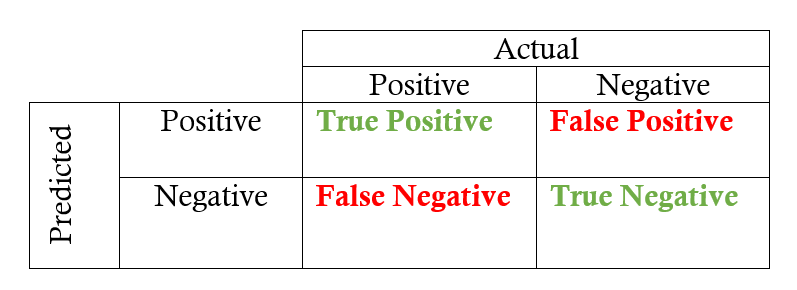
\includegraphics[scale=0.3]{resources/3/confusionMatrix}
\end{description}
\item ``Confusion Circle''
\begin{description}
\item \includegraphics[scale=0.35]{resources/3/confusionCircle}
\end{description}
\item Loan Threshold
\begin{description}
\item 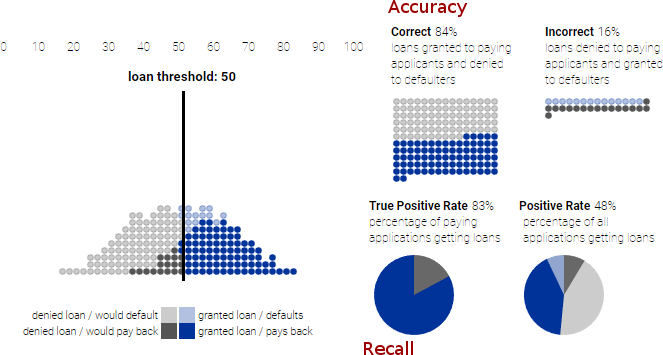
\includegraphics[scale=0.57]{resources/4/loanML4}
\end{description}
\end{itemize}
%
\subsection{Recall}
\begin{enumerate}
\item Recall ($\equiv$ True Positive Rate) is defined as the ability of a model to find all relevant cases within the dataset.
\end{enumerate}
\begin{tabular}{|l|l|l|l|}
\hline
2. & 3. & 4.\\ 
$= \frac{\texttt{TP}}{\texttt{TP} + \texttt{FN}}$ & $= \frac{
\includegraphics[scale=0.1]{resources/3/confusionCircleTP}}{
\includegraphics[scale=0.1]{resources/3/confusionCircleTP+FN}}$ & $= \frac{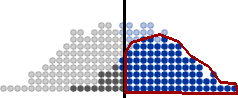
\includegraphics[scale=0.6]{resources/4/loanTP}}{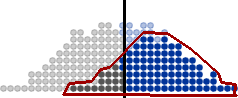
\includegraphics[scale=0.6]{resources/4/loanTP+FN}}$\\ \hline
\end{tabular}
%
\subsection{Precision}
\begin{enumerate}
\item Ability of the model to find only relevant cases within the dataset
\end{enumerate}
\begin{tabular}{|l|l|l|l|}
\hline
2. & 3. & 4.\\ 
$= \frac{\texttt{TP}}{\texttt{TP} + \texttt{FP}}$ & $= \frac{
\includegraphics[scale=0.1]{resources/3/confusionCircleTP}}{
\includegraphics[scale=0.1]{resources/3/confusionCircleTP+FP}}$ & $= \frac{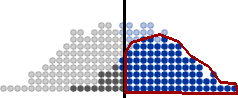
\includegraphics[scale=0.6]{resources/4/loanTP}}{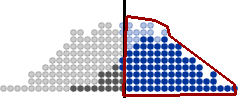
\includegraphics[scale=0.6]{resources/4/loanTP+FP}}$\\ \hline
\end{tabular}
%
\subsection{F1}
\begin{enumerate}
\item F1-Score, the harmonic mean of recall and precision, a metric from 0 (worst) to 1 (best), used to evaluate the accuracy of a model by taking recall and precision into account 
\end{enumerate}
\begin{tabular}{|l|l|l|l|}
\hline
2. & 3. & 4.\\ 
- & - & - \\ \hline
\end{tabular}
\begin{description}
\item $=2*\frac{\texttt{precision} * \texttt{recall}}{\texttt{precision}+\texttt{recall}}$
\item Compared to the simple average (of recall and precision), the harmonic mean punishes extreme values (e.g. precision 1.0 and recall 0.0 $\rightarrow$ average 0.5, but F1 $= 0$)
\end{description}

%
%
%
\newpage
\section*{Questions}
\begin{itemize}
%
\item \colorbox{yellow}{Q:} Should I ask Aaron how he would like us to work together? I'm not sure how he meant it.
\begin{description}
\item \colorbox{orange}{A:} 
\end{description}
%
\item \colorbox{yellow}{Q:} In what situations exactly do we want to optimize the threshold in the context of user centered threshold optimization?
\begin{description}
\item \colorbox{orange}{A:} 
\end{description}
%
\item \colorbox{yellow}{Q:} VPN recommendation?
\begin{description}
\item \colorbox{orange}{A:} 
\end{description}
%
\end{itemize}
\end{document}